\documentclass[
10pt, % Main document font size
a4paper, % Paper type, use 'letterpaper' for US Letter paper
oneside, % One page layout (no page indentation)
%twoside, % Two page layout (page indentation for binding and different headers)
headinclude,footinclude, % Extra spacing for the header and footer
BCOR5mm, % Binding correction
]{scrartcl}

\usepackage{listings}
\usepackage{color}
%\usepackage{biblatex}

\definecolor{dkgreen}{rgb}{0,0.6,0}
\definecolor{gray}{rgb}{0.5,0.5,0.5}
\definecolor{mauve}{rgb}{0.58,0,0.82}

\lstset{frame=tb,
	language={Haskell},
	aboveskip=3mm,
	belowskip=3mm,
	showstringspaces=false,
	columns=flexible,
	basicstyle={\small\ttfamily},
	numbers=none,
	numberstyle=\tiny\color{gray},
	keywordstyle=\color{blue},
	commentstyle=\color{dkgreen},
	stringstyle=\color{mauve},
	breaklines=true,
	breakatwhitespace=true,
	tabsize=3
}

\usepackage{german}

\usepackage{filecontents}
%usepackage[utf8]{inputenc}
%\usepackage{geometry}
\usepackage[german,onelanguage,linesnumbered, ruled]{algorithm2e}
\SetAlFnt{\small}
\SetAlCapFnt{\large}
\SetAlCapNameFnt{\large}
%\usepackage{algpseudocode}


%%%%%%%%%%%%%%%%%%%%%%%%%%%%%%%%%%%%%%%%%
% Arsclassica Article
% Structure Specification File
%
% This file has been downloaded from:
% http://www.LaTeXTemplates.com
%
% Original author:
% Lorenzo Pantieri (http://www.lorenzopantieri.net) with extensive modifications by:
% Vel (vel@latextemplates.com)
%
% License:
% CC BY-NC-SA 3.0 (http://creativecommons.org/licenses/by-nc-sa/3.0/)
%
%%%%%%%%%%%%%%%%%%%%%%%%%%%%%%%%%%%%%%%%%

%----------------------------------------------------------------------------------------
%	REQUIRED PACKAGES
%----------------------------------------------------------------------------------------

\usepackage[
nochapters, % Turn off chapters since this is an article        
beramono, % Use the Bera Mono font for monospaced text (\texttt)
eulermath,% Use the Euler font for mathematics
pdfspacing, % Makes use of pdftex’ letter spacing capabilities via the microtype package
dottedtoc % Dotted lines leading to the page numbers in the table of contents
]{classicthesis} % The layout is based on the Classic Thesis style

\usepackage{arsclassica} % Modifies the Classic Thesis package

\usepackage[T1]{fontenc} % Use 8-bit encoding that has 256 glyphs

\usepackage[utf8]{inputenc} % Required for including letters with accents

\usepackage{graphicx} % Required for including images
\graphicspath{{Figures/}} % Set the default folder for images

\usepackage{enumitem} % Required for manipulating the whitespace between and within lists

\usepackage{lipsum} % Used for inserting dummy 'Lorem ipsum' text into the template

\usepackage{subfig} % Required for creating figures with multiple parts (subfigures)

\usepackage{amsmath,amssymb,amsthm} % For including math equations, theorems, symbols, etc

\usepackage{varioref} % More descriptive referencing

%----------------------------------------------------------------------------------------
%	THEOREM STYLES
%---------------------------------------------------------------------------------------

\theoremstyle{definition} % Define theorem styles here based on the definition style (used for definitions and examples)
\newtheorem{definition}{Definition}

\theoremstyle{plain} % Define theorem styles here based on the plain style (used for theorems, lemmas, propositions)
\newtheorem{theorem}{Theorem}

\theoremstyle{remark} % Define theorem styles here based on the remark style (used for remarks and notes)

%----------------------------------------------------------------------------------------
%	HYPERLINKS
%---------------------------------------------------------------------------------------

\hypersetup{
%draft, % Uncomment to remove all links (useful for printing in black and white)
colorlinks=true, breaklinks=true, bookmarks=true,bookmarksnumbered,
urlcolor=webbrown, linkcolor=RoyalBlue, citecolor=webgreen, % Link colors
pdftitle={}, % PDF title
pdfauthor={\textcopyright}, % PDF Author
pdfsubject={}, % PDF Subject
pdfkeywords={}, % PDF Keywords
pdfcreator={pdfLaTeX}, % PDF Creator
pdfproducer={LaTeX with hyperref and ClassicThesis} % PDF producer
} % Include the structure.tex file which specified the document structure and layout

\hyphenation{Fortran hy-phen-ation} % Specify custom hyphenation points in words with dashes where you would like hyphenation to occur, or alternatively, don't put any dashes in a word to stop hyphenation altogether

%----------------------------------------------------------------------------------------
%	TITLE AND AUTHOR(S)
%----------------------------------------------------------------------------------------

\title{\normalfont\spacedallcaps{Projektaufgabe AE}} % The article title

\subtitle{Remove Duplicates - Spotify playlist cleaner} % Uncomment to display a subtitle

\author{\spacedlowsmallcaps{Raphael Drechsler}} % The article author(s) - author affiliations need to be specified in the AUTHOR AFFILIATIONS block

\date{} % An optional date to appear under the author(s)

%----------------------------------------------------------------------------------------

\begin{document}

%----------------------------------------------------------------------------------------
%	HEADERS
%----------------------------------------------------------------------------------------

\renewcommand{\sectionmark}[1]{\markright{\spacedlowsmallcaps{#1}}} % The header for all pages (oneside) or for even pages (twoside)
%\renewcommand{\subsectionmark}[1]{\markright{\thesubsection~#1}} % Uncomment when using the twoside option - this modifies the header on odd pages
\lehead{\mbox{\llap{\small\thepage\kern1em\color{halfgray} \vline}\color{halfgray}\hspace{0.5em}\rightmark\hfil}} % The header style

\pagestyle{scrheadings} % Enable the headers specified in this block

%----------------------------------------------------------------------------------------
%	TABLE OF CONTENTS & LISTS OF FIGURES AND TABLES
%----------------------------------------------------------------------------------------

%\maketitle % Print the title/author/date block
{ \centering
{ \par}\
 \linebreak
\linebreak 
\linebreak
\linebreak
\linebreak
%\centering

\includegraphics[width=0.55\columnwidth]{htwLogo} 
\linebreak
\linebreak
\linebreak
\linebreak 
 % inline
{\fontsize{14}{16}\selectfont \center Fakultät Informatik, Mathematik und\\Naturwissenschaften\\Studiengang Informatik Master\par}\
 \linebreak
{\fontsize{18}{20}\selectfont \center \textbf{Projektarbeit zur Vorlesung Computermusik}\par}\
{\fontsize{20}{22}\selectfont \center \textbf{BrandtBrauerFrick.hs} \par}\
\linebreak
\linebreak
\linebreak
\linebreak 
\linebreak
\linebreak 
\linebreak 
{\fontsize{14}{16}\selectfont  \begin{tabular}{rl}
 	\textbf{Autoren:} & Nico Mehlhose, Raphael Drechsler\\ 
 	\textbf{Abgabedatum:} & 03.02.2019 \\ 
 \end{tabular}
\par}
\par}
\pagebreak
\setcounter{tocdepth}{2} % Set the depth of the table of contents to show sections and subsections only

\tableofcontents % Print the table of contents
%\listoffigures % Print the list of figures
%\listoftables % Print the list of tables




%----------------------------------------------------------------------------------------

\newpage % Start the article content on the second page, remove this if you have a longer abstract that goes onto the second page

%----------------------------------------------------------------------------------------
%	INTRODUCTION
%----------------------------------------------------------------------------------------
\section{Abstract}\
\textit{Abschnitt bearbeitet von: Raphael Drechsler}\\

\noindent \textbf{BrandtBrauerFrick.hs}

\noindent Brandt Brauer Frick ist ein Techno-Projekt aus Berlin.
Die Basis des Projekts bilden Klänge aus dem Instrumentarium der
klassischen Musik, welche anfangs gesampelt, später in einem zehnköpfigen
Ensemble auch live vorgeführt wurden.\cite{Wiki}\\ 

\noindent Ziel des Projektes:\\
Die Umsetzung des Songs ''Pretend'' von Brandt Brauer Frick entweder in
Tidal oder Euterpea. Eine online verfügbare Live-Aufführung \cite{YT1} soll dabei als Referenz dienen. Bei der Umsetzung soll auch Wert auf die Nachbildung der echten Instrumente und deren teilweise Zweckentfremdung gelegt werden.\\

\noindent Herausforderungen:
\begin{itemize}
	\itemsep0em
	\item Evaluation ob Tidal\cite{Tidal} oder Euterpea\cite{Euterpea} genutzt werden soll:
	\item Untersuchung der Frage ob klassische Klänge am ehesten in Euterpea oder
	Tidal nutzbar sind. (Durch repetitiven Charakter des Liedes würde sich Tidal zur
	Live-Vorführung eignen)
	\item Analyse der einzelnen musikalischen Bausteine und deren Implementierung.
	\item Zusammenfügen der erarbeiteten Bausteine zu einer Performance.
\end{itemize}

\section{Umsetzung in Tidal oder Euterpea}\
\textit{Abschnitt bearbeitet von: Nico Mehlhose}\\

\noindent Dieses Thema soll sich um die Evaluation zwischen Tidal und Eutherpea handeln. Bevor es zu der Evaluation kommt, werden die eben genannten
Programme kurz erklärt.\\
Tidal ist eine Open Source Software mit deren Hilfe es möglich ist Musikpatterns per Code zu generieren. Tidal benutzt den Synthesizer \textit{SuperCollider}.\cite{Tidal}\\
Der SuperCollider, ebenfalls eine Open Source Software, ist ein Audio-Synthesizer. Dabei können eigene Klänge oder Instrumente mithilfe von unterschiedlichen Oszilatoren, Filtern
und anderen Hilfsmitteln des SuperColliders erstellt werden. \cite{SC}\\
Euterpea ist ein in Haskell eingebettetes Programm, welches durch Code u. a. Musik erzeugt, algorithmische Komposition und Sound Synthese ermöglicht.\cite{Euterpea}\\
Im Endeffekt ist unsere Auswahl des Programmes auf Tidal gefallen. In diese Entscheidung ist der Programmieraufwand, vorhandenen Informationen
und die Möglichkeit den Synthesizer zu erweitern mit eingeflossen.\\
Bei dem Programmieraufwand wird sehr schnell klar, dass das sehr repetetive Lied \textit{Pretent} von BrandBrauerFrick für Tidal besser geeignet ist als für Euterpea, da in Tidal die Musikpatterns immer in einem loop abgespielt werden. In Eutherpea kann dieser Effekt nur durch zusätzlichen Programmieraufwand erreicht werden.\\ 
Bei den vorhandenen Informationen zu dem Musikstück stellt sich heraus, dass keine offiziellen Notenblätter für das Lied Online existieren, wodurch Euterpea etwas an Bedeutung verliert, da Euterpea für genaue Notenbestimmungen perfekt geeignet wäre. Durch die absenz dieses Faktors, kann das selbe Maß an Genauigkeit auch mit Tidal erreicht werden.\\
Der Letzte und für uns wichtigste Punkt war die Erweiterbarkeit der Sounds. Die Wichtigkeit darin besteht in der entfremdeten Benutzung der Musikinstrumente in dem Lied.
In Eutherpea haben wir nach einiger Recherche keinen weg gefunden Sounds hinzuzufügen um diese später zu verwenden. In Tidal existiert diese Möglichkeit mittels
dem Befehl \verb|~dirt.loadSoundFiles(”full/path/to/directory/*”)|. Mit diesem Befehl lässt sich ein Verzeichnis in Tidal integrieren. Anschließend können die Sounds beim Programmieren mit dem Ordnernamen benutzt werden.\cite{tidcy}
\section{Eigenschaften des Stücks Pretend und dessen globale Struktur}\
\textit{Abschnitt bearbeitet von: Raphael Drechsler}\\

\noindent Die in der Live vorgeführte Version \cite{YT1} hat eine ungefähre Dauer von 7 Minuten, 15 Sekunden. Die Angabe erfolgt ungefähr, da die Aufnahme nicht mit dem ersten Takt beginnt\\
Per Gehör ließ sich feststellen, dass das Stück in der Tonart Gm steht.\\
Über ein BPM-Measuring-Tool \cite{tempo} wurde ein Tempo von 130bpm ermittelt. In Tidal wird somit der folgende Code zur Tempo-Einstellung benötigt. 
\begin{lstlisting}
setcps (130/60/4)
\end{lstlisting}

\noindent Die Globale Struktur des Liedes, also die Zeitliche Abfolge der Figuren der einzelnen Instrumente, wurde per Gehör analysiert. Dabei wurde ebenfalls die Live-Version des Liedes als Untersuchungsgegenstand verwendet. Um das Ergebnis zu visualisieren, wurden in Logic Pro\cite{Logic} (einer digital Audio-Workstation der Firma Apple) für die jeweiligen Figuren leere MIDI-Regionen innerhalb der 237 Takte erzeugt.
Anschließend wurde das Resultat per Screenshot aufgenommen und die einzelnen Figuren mit F1,F2,... für die jeweilige Figur beschriftet. Zur besseren Verständigung darüber, wo man sich innerhalb der globalen Struktur befindet wurde das Lied in 10 Parts unterteilt. Diese wurden mit P1,P2,...,P10 beschriftet.\\
Für die ersten vier Takte wurde bei der Erstellung der MIDI-Regionen eine Annahme getroffen.

\begin{figure}[h]
	\centering 
	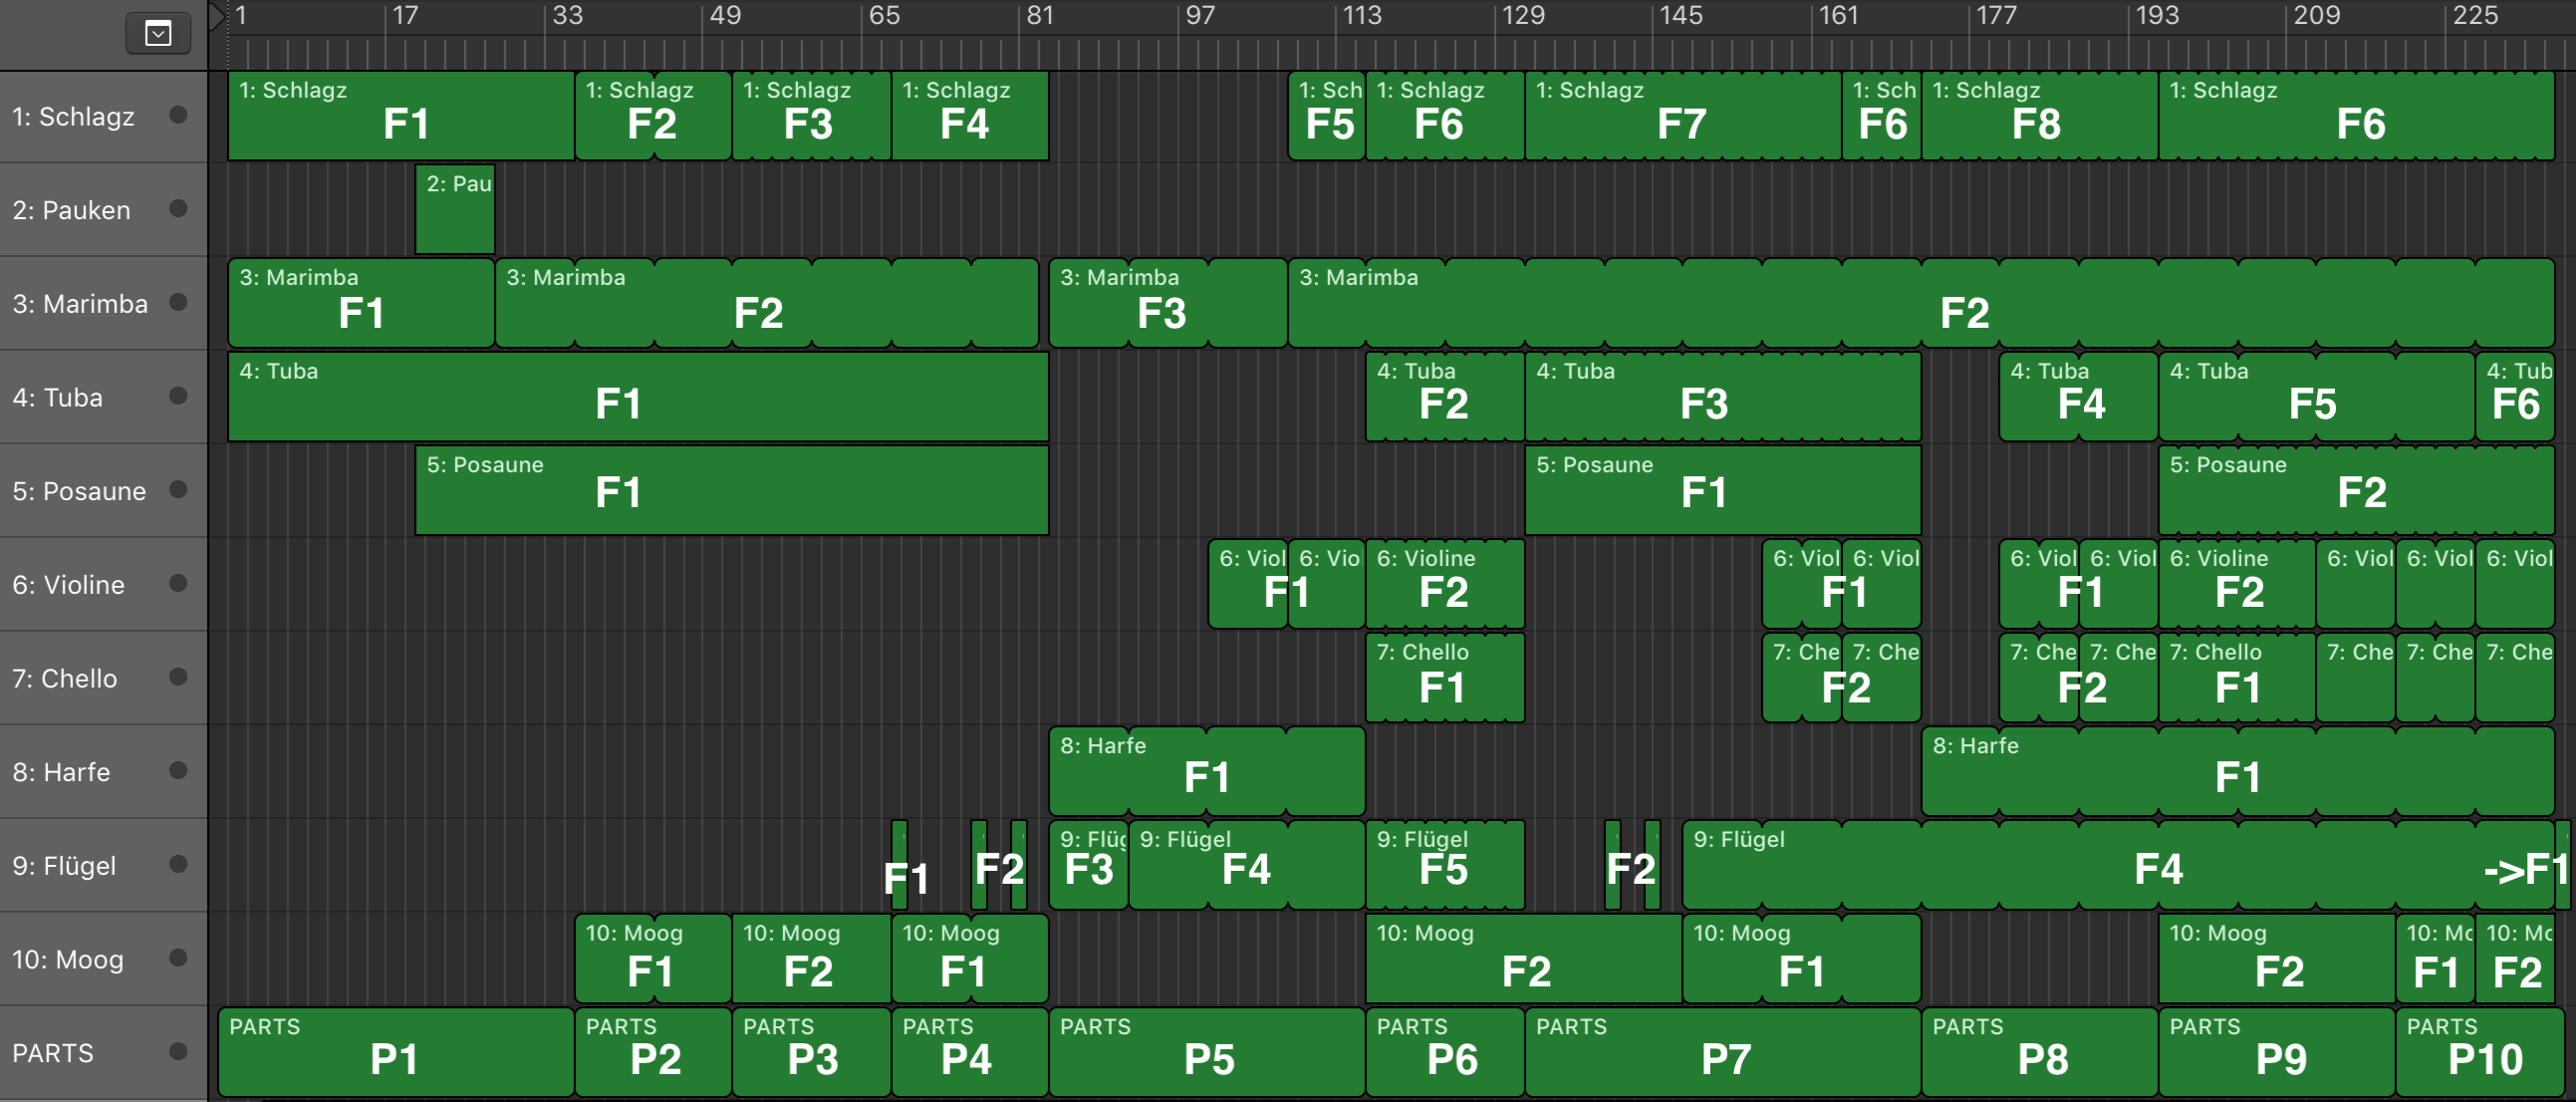
\includegraphics[width=0.99\columnwidth]{GlobaleStrukturMarkiert} 
	\caption{Globale Struktur dargestellt als leere MIDI-Regionen in Logic Pro mit Beschriftung der Figuren}
\end{figure}

\noindent Es wurde ebenfalls versucht die Abfolge mithilfe eines freien Notations-Programmes in einer Partitur darzustellen. Jedoch erwies sich die obige Darstellung als kompakter und ausreichend.

\section{Analyse und Synthese der einzelnen Instrumente}\
\textit{Abschnitt bearbeitet von: Raphael Drechsler}\\

\noindent Im folgenden Abschnitt sollen neun der zehn Instrumente synthetisiert werden. Da die Pauken auf einer ähnlichen Frequenz klingen wie die Bass-Drum und Moog-Synthesizer sind diese nur sehr schwer aus dem Stück herauszuhören. Durch diesen Umstand und mit der Absicht das fertig synthetisierte Stück nicht zu überladen wurde daher beschlossen auf Analyse und Synthese der Pauken zu verzichten.\\

\noindent Wie in der globalen Struktur (siehe Abb. 1) zu erkennen ist, existieren in den meisten Fällen pro Instrument mehrere Figuren. Die folgenden Arbeitsschritte sollen daher pro Instrument und Figur erfolgen.

\paragraph{Analyse der gespielten Tonhöhen und Rhythmen.}  Diese Analyse erfolgt per Gehör. Untersucht wird dabei die Live-Version\cite{YT1} des Stückes. Für Figuren, die besonders schwierig herauszuhören sind, da z.B. das Instrument nur sehr schwer hörbar ist, werden zusätzlich eine ähnliche Studio-Version\cite{YT2} sowie eine früher Variante\cite{YT3} des Liedes für die Untersuchung herangezogen.	Das Ergebnis der Analyse soll hier als Text, welcher die Figur beschreibt und/oder mithilfe von Noten dargestellt werden. 

\paragraph{Synthese von Tonhöhe und Rhythmus} Die analysierten Tonhöhen und Rhythmen sollen als Tidal Code umgesetzt werden. Dabei wird kein gesteigerter Wert auf die Auswahl eines passenden Klanges gelegt. Im Vordergrund der Betrachtung steht, dass der umgesetzte Code den analysierten Tonhöhen und Rhythmen entspricht. Vereinzelt soll hierbei auf zu überwindende Herausforderungen und genutzte Funktionen eingegangen werden.

\paragraph{Klanganalyse} Per Gehör soll das Klangbild des Instrumentes in der speziellen Figur sowie die Wirkung, welche durch die Figur beim Hörer erzeugt wird, untersucht werden. 

\paragraph{Anpassung der Klangsynthese} Unter Berücksichtigung des analysierten Klangbildes und des bereits vorliegenden Tidal-Codes soll nun die Art der Klangsynthese derart angepasst werden, dass die beschriebene klangliche Wirkung erzielt wird. Mögliche Arten der Anpassung sind dabei die Auswahl von Tidal-Instrumenten, Einbinden von fremden und selbst aufgenommenen Samples sowie das Erstellen eines SuperCollider-Instrumentes.\\

\noindent Auf diesem Wege sollen die Figuren aller Instrumente als ausführbarer Tidal-Code mit erwünschter klanglicher Wirkung entstehen.
Das Verbinden der einzelnen Figuren zu einem live vorführbaren Stück soll in \textit{Kapitel 5 - Performance} beschrieben werden. 


%
%\subsection{Instrument 0: Was ist pro Instrument TODO?}
%{\color{red}\textbf{TODO}}: Nach Bearbeitung Hilfskapitel entfernen.\\
%
%Raph.\\
%Welche Figuren?
%- Welche Wirkung?
%- Welche Noten?\\
%
%Nico\\
%Wie klingt das Instrument?\\
%- Wie klingt das live? Einzelne Bestandteile? (Marimba gespielt mit Holzsticks und verschiedene Kuhglocken)
%- Wie klingt das in welcher Figur? (zB. BD laut, leise)
%- Welchen Klang wählen (evaluation - SD-Instrument nutzbar?, WAV suchen/selber aufnehmen, Instrument coden)\\

\subsection{Instrument 1: Schlagzeug}
\subsubsection{Figuren}
\textit{Abschnitt bearbeitet von: Raphael Drechsler}\\

\noindent \textbf{Figur 1}\\
Herausgehört wurde das folgende Muster. Die Note \textit{A} steht dabei für die Bass-Drum, Note \textit{Dis} für die High-Hat.
\begin{figure}[h]
	\centering 
	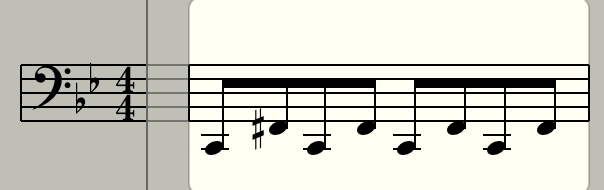
\includegraphics[width=0.3\columnwidth]{Drum_Fig1} 
	\caption{Schlagzeug Figur 1}
\end{figure}

\noindent Um in Tidal pro Takt eine Figur mit 4 Schlägen auf die Bass-Drum und 4 Schlägen auf die High-Hat im Wechsel zu realisieren, lässt sich eine Kombination von Gruppierung und Wiederholung\cite{tid1} verenden:
\begin{lstlisting}
d1 $ sound "[bd hh]*4"
\end{lstlisting}

\noindent \textbf{Figur 2}\\
Herausgehört wurde eine Figur über 8 Takte. Dabei werden in Takt 3,7 und 8 wie nachfolgend notiert Fills auf der High-Hat gespielt.\\
\begin{figure}[h]
	\centering 
	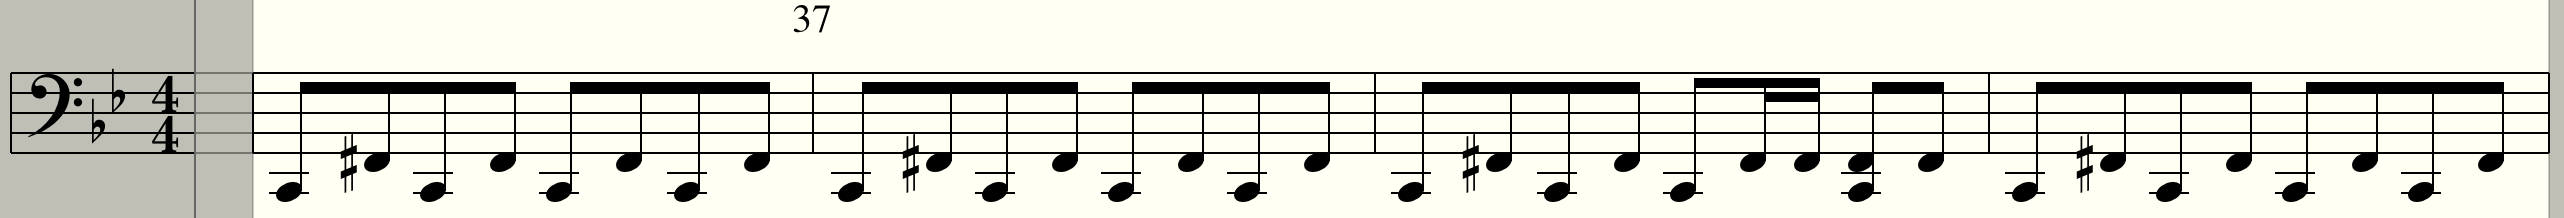
\includegraphics[width=0.8\columnwidth]{Drums_Fig2A} 
	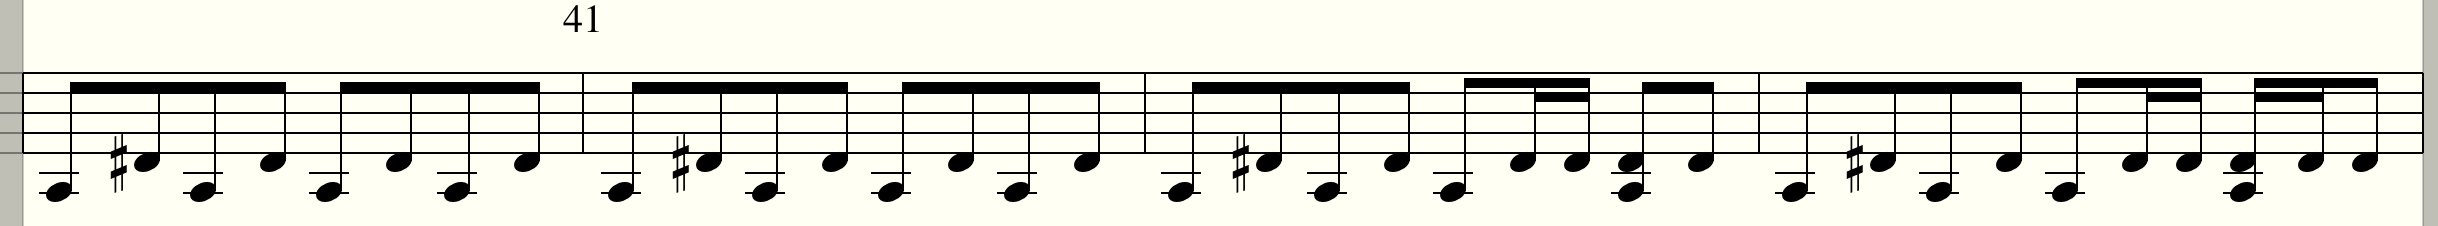
\includegraphics[width=0.8\columnwidth]{Drums_Fig2B} 
	\caption{Schlagzeug Figur 2}
\end{figure}

\noindent Die Umsetzung in Tidal der einzelnen Takte ohne Fills erfolgt analog zu Figur 1. In den Takten mit Fills werden auf einige Zählzeiten Bass-Drum und High-Hat gleichzeitig gespielt. Dies kann in Tidal durch die Nutzung von   \verb1stack1 \cite{tid2} umgesetzt werden. Über den \verb1cat1-Ausdruck\cite{tid3} werden die acht Figuren hintereinander gespielt, was den Cycle auf die gewünschte Länge von acht Takten verlängert. Es ergibt sich folgender Code.

\begin{lstlisting}
d1 $  cat [
sound "[[bd hh]*4]",
sound "[[bd hh]*4]",
stack [ sound "[bd ~]*4", sound "[~ hh ~ hh][~ [hh hh] hh hh]" ],
sound "[[bd hh]*4]",
sound "[[bd hh]*4]",
sound "[[bd hh]*4]",
stack [ sound "[bd ~]*4", sound "[~ hh ~ hh][~ [hh hh] hh hh]" ],
stack [ sound "[bd ~]*4", sound "[~ hh ~ hh][~ [hh hh] [hh hh] hh]" ]
]
\end{lstlisting}

\noindent \textbf{Figur 3}\\
Herausgehört wurde die folgende Figur mit zwei Takten Länge. Die Note \textit{Fes} steht dabei für eine geöffnete High-Hat.
\begin{figure}[h]
	\centering 
	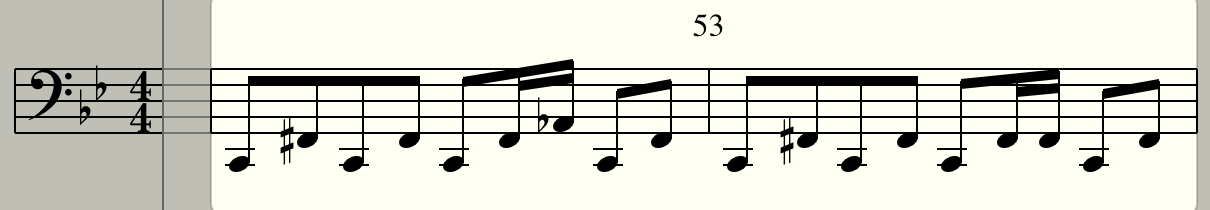
\includegraphics[width=0.5\columnwidth]{Drums_Fig3} 
	\caption{Schlagzeug Figur 1}
\end{figure}

\noindent In Tidal wurde die Figur hintereinander in Gruppierungen geschrieben und per \verb1slow 21\cite{tid4} auf die Länge von zwei Takten gestreckt.
\begin{lstlisting}
d1 $  slow 2 $ sound "[bd hh bd hh][bd [hh ho] bd hh] [bd hh bd hh][bd [hh hh] bd hh]"
\end{lstlisting}

\noindent \textbf{Figur 4}\\
Analog zu Figur 1. Dazu kommen zyklische Bewegung auf der Rim (Rand der Snare-Drum).
Die Figur ließ sich nur schwer durch Heraushören bestimmen. Es wurden daher 5 Schläge auf die Rim pro Takt als Annahme getroffen, wobei aller 2 Takte der letzte Schlag ausgelassen wird.\\

\noindent Dies realisiert der folgende Tidal-Code.
\begin{lstlisting}
d1 $ stack [
sound "[bd hh]*4",
cat[sound "[rm rm rm rm rm]", sound "[rm rm rm rm ~]"] 
]
\end{lstlisting}

\noindent \textbf{Figur 5}\\
Nur die zyklische Rimclick-Bewegung aus Figur 4.
\begin{lstlisting}
d1 $ cat[sound "[rm rm rm rm rm]", sound "[rm rm rm rm ~]"]
\end{lstlisting}

\noindent \textbf{Figur 6 und 7}\\
Figur 6 wie Figur 4 und Figur 7 wie Figur 3. Jeweils kräftiger gespielt. Dies wird später in der Performance mit einem \verb1# gain1-Ausdruck\cite{tid5} zum Regulieren der Lautstärke des gespielten Samples umgesetzt.\\

\noindent \textbf{Figur 8}\\
Wie Figur 4 aber ohne Bass-Drum.
\begin{lstlisting}
d1 $ stack [
sound "[~ hh]*4" ,
cat[sound "[rm rm rm rm rm]", sound "[rm rm rm rm ~]"] 
]
\end{lstlisting}

\subsubsection{Klangbild}
\textit{Abschnitt bearbeitet von: Nico Mehlhose}\\

\noindent Art der Synthetisierung: Da Bass Drum und High Hat normal gespielt werden können die Sounds aus dem Supercollider 
mit minimaler Anpassung benutzt werden. Lediglich die Rim aus Figur 4 muss, wegen ihres hölzernen Sounds, selbst 
aufgenommen werden.\\


\noindent \textbf{Figur 1}\\
Sound BD: Die Bass Drum wird mit zunehmender Dauer lauter gespielt.\\
Sound HH: Auch die HH wird Anfangs nur sanft angespielt aber mit zunehmender Zeit lauter.\\
Problem: Bass Drum und High Hat müssen mit zunehmender Vorführungszeit lauter werden.\\ 
Lösung: Die Lautstärkensteigerung der Schlagzeugs wird live, mittels der Erhöhung des \textit{gain}-Parameters, realisiert.
\begin{lstlisting}
d1 $ sound "[bd hh]*4" #midinote 58 #gain 0.9
\end{lstlisting}
\noindent \textbf{Figur 2}\\
Sound: Das Schlagzeug wird in dieser Figur, bis auf die Lautstärkensteigerung, analog zu Figur 1 gespielt. In dieser Figur ist die Lautstärke gleichbleibend.\\
\noindent \textbf{Figur 3}\\
Sound: Die Bass-Drum wird etwas schwächer angespielt um einen zu starken Bass zu vermeiden und um nicht dominant zu wirken. Selbiges gilt für die High Hat. Dies wird in der Performance berücksichtigt.
\noindent \textbf{Figur 4}\\
Sound: In Figur 4 wurde eine hölzern klingende Rim hinzugefügt. Diese ist nur sehr dezent im Klangbild zu erkennen.
Lösung: Die hölzern klingende Rim wurde durch einen Schlag eines Bleistiftes auf eine kleine hölzerne Kiste erzeugt. \verb|room| soll der Rim noch einen hallenden Charakter geben, da der aufgenommene Sound diesen nicht besessen hat.
 \begin{lstlisting}
d1 $ stack [
sound "[bd hh]*4"  #midinote 58 #gain 1.0,
cat[
  sound "[Rim Rim Rim Rim Rim]",
  sound "[Rim Rim Rim Rim ~]"
  ] #room 0.15 #orbit 1 #gain 1.5
]
\end{lstlisting}
\noindent \textbf{Figur 5}\\
Sound: In dieser Figur wird lediglich die hölzerne Rim gespielt. Die Rim wird analog zu Figur 4 gespielt.\\
\noindent \textbf{Figur 6 und 7}\\
Sound: Figur 6 wird wie Figur 4 gespielt und Figur 7 wie Figur 3. In beiden Fällen sind 6 und 7 nur lauter gespielt, was über den \verb|Gain|-Befehl realisiert wird.\\
\noindent \textbf{Figur 8}\\
Sound: Die letzte Figur des Schlagzeugs ist für \grqq die Ruhe vor dem Sturm\grqq zuständig, welche kurz vor dem zweiten Hauptteil zu hören ist. Dabei sieht diese Figur so aus
wie Figur 4, jedoch fehlt die Bass Drum was für die \grqq Ruhe\grqq sorgt.\\
Lösung:
\begin{lstlisting}
d1 $ stack [
  sound "[~ hh]*4" #midinote 58 #gain 1.3,
  cat[
    sound "[Rim Rim Rim Rim Rim]",
    sound "[Rim Rim Rim Rim ~]"] #gain 1.0
]
\end{lstlisting}

\subsection{Instrument 2: Pauke}
Wird, wie oben erwähnt, nicht synthetisiert.

\subsection{Instrument 3: Marimba}
\subsubsection{Figuren}
\textit{Abschnitt bearbeitet von: Raphael Drechsler}\\

\noindent \textbf{Figur 1}\\
Die Tonhöhe war per Gehör nicht genau differenzierbar. Es wurde folgende Annahme getroffen.
\begin{figure}[h]
	\centering 
	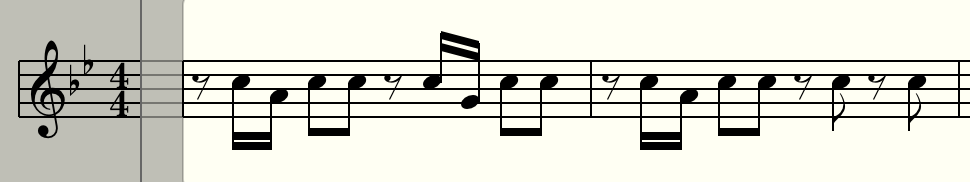
\includegraphics[width=0.5\columnwidth]{Marimba_Fig1} 
	\caption{Marimba Figur 1}
\end{figure}

\noindent Die Tonhöhe des Sounds \verb|glasstrap| wurde mithilfe des \verb|midinote|-Ausdrucks \cite{tid6} auf die jeweils gewünschte Tonhöhe geändert.
\begin{lstlisting}
d1 $ slow 2 $ midinote "[~ [51 49] 51 51][~ [51 46] 51 51][~ [51 49] 51 51][~ 51 ~ 51]" # s "glasstap"
\end{lstlisting}


\noindent \textbf{Figur 2}\\
In der Live-Version des Liedes ist im Video zu erkennen, dass auf der Marimba Kuhglocken (8 oder 10 Stück) in verschiedenen Tonhöhen liegen. Diese werden in der zweiten Figur auf die in der folgenden Abbildung gezeigten Zählzeit angespielt. Dabei wird Immer eine andere Tonhöhe gespielt. Das Muster in welcher Reihenfolge die Glocken gespielt werden wurde nicht weiter analysiert. Stattdessen soll das Anspielen der Glocken zur Vereinfachung randomisiert werden.
\begin{figure}[h]
	\centering 
	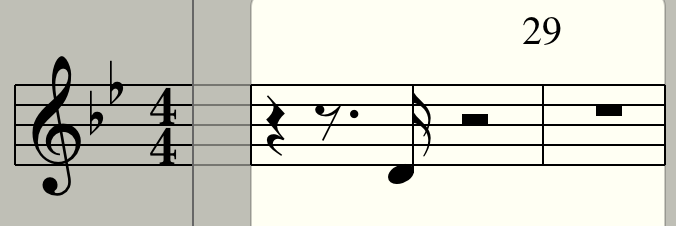
\includegraphics[width=0.25\columnwidth]{Marimba_Fig2} 
	\caption{Marimba Figur 2}
\end{figure}

\noindent Der Ausdruck \verb|irand 10| \cite{tid7} liefert einen zufälligen int-Wert von 0 bis einschließlich 9 zurück. Dieser Wert verändert in Verbindung mit dem \verb|# speed|-Ausdruck\cite{tid8} die Abspielgeschwindigkeit des \verb|can|-Samples und damit dessen Tonhöhe. So werden 9 verschiedene Kuhglocken simuliert.
\begin{lstlisting}
d1 $ stack [
slow 2 $ midinote "[~ [51 49] 51 51][~ [51 46] 51 51][~ [51 49] 51 51][~ 51 ~ 51]" # s "glasstap",
slow 2 $ midinote "[~[~~~60]~~][]" # s "can" # speed (1 + (irand 10)*0.2)
]
\end{lstlisting} 

\noindent \textbf{Figur 3}\\
Es wurde folgende Figur per Gehör ermittelt. Dabei sind die Tonhöhen wie in Figur 1 angenommen.
\begin{figure}[h]
	\centering 
	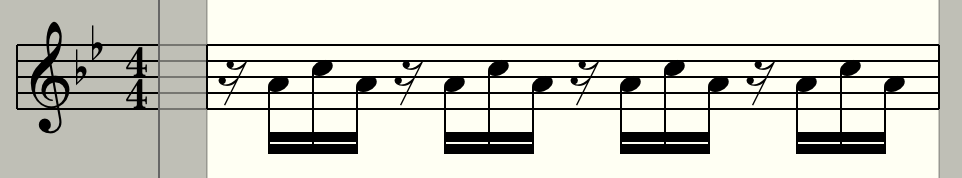
\includegraphics[width=0.5\columnwidth]{Marimba_Fig3} 
	\caption{Marimba Figur 3}
\end{figure}

\noindent Umsetzung in Tidal:
\begin{lstlisting}
d1 $ midinote "[~ 49 51 49]*4" # s "glasstap"
\end{lstlisting}


\subsubsection{Klangbild}
\textit{Abschnitt bearbeitet von: Nico Mehlhose}\\

\noindent Bestandteile der Marimba: Eine Marimba, wobei Kuhglocken zum zufälligem Anspielen enthalten sind.\\
Art der Synthetisierung: Da keine hölzernen Klänge im SuperCollider enthalten sind müssen diese selbst erstellt werden. Dies geschieht mittels 
einem von \textit{SuperCollider Code} stammenden Code.\cite{Marimba}\\
Folgender Code wurde leicht abgewandelt, sodass er unseren Anforderungen entspricht:
\begin{lstlisting}
(
SynthDef(\bell, {
	|fs=1, t60=1, pitchy=1, amp=0.25, gate=1|
	var sig, exciter;
	//exciter = Impulse.ar(0);
	exciter = WhiteNoise.ar() * EnvGen.ar(Env.perc(0.001, 0.05), gate) * 0.25;
	sig = Klank.ar(
		`[
			[1, 2, 2.803, 3.871, 5.074, 7.81, 10.948, 14.421],   // freqs
			[1, 0.044, 0.891, 0.0891, 0.794, 0.1, 0.281, 0.079], // amplitudes
			[1, 0.205, 1, 0.196, 0.339, 0.047, 0.058, 0.047]*t60     // ring times
		],
		exciter,
		freqscale:fs*pitchy);
	sig = FreeVerb.ar(sig) * amp;
	DetectSilence.ar(sig, 0.001, 0.5, doneAction:2);
	Out.ar(0, sig!2);
}).add
)


(
Pbind(
	\instrument, \bell,
	\fs, 60.midicps,
	\t60, 0.45,
	\pitchy, 1.75,
	\dur, 0.25
).play;)
\end{lstlisting}
Wobei der erste Teil des Codes einen Ton erzeugt welcher Vergleichbar ist mit dem Kratzen auf einem Mikrofon.\\
Der zweite Teil ändert den ersten Sound so ab, sodass dieser mehr hölzern klingt.\\
Als nächstes muss dieser Sound aus dem SuperCollider aufgenommen werden. Dies wird mit dem Befehl \textit{Server.default.record;} umgesetzt.\cite{tidcy}\\
Der dritte Schritt war das Zuschneiden der Audisamples. Dazu wurde Audacity benutzt. Audacity ist ein kostenlosen Audioschnitt-, Editierungs- und Aufnahmeprogramm.\cite{Auda} Im Anschluss kann dann der Code für die einzelnen Figuren angepasst werden.\\
		
\noindent \textbf{Figur 1}\\
Sound : Die Marimba wird am Anfang des Stücks relativ dominant, im Gegensatz zu den restlichen Instrumenten, gespielt.Dieser Effekt entsteht durch den \verb|Gain|-Opperator in der Schlagzeugfigur 1.\\
Lösung:
\begin{lstlisting}
d1 $ slow 2 $ midinote "[~ [65 63] 65 65][~ [65 60] 65 65][~ [65 63] 65 65][~ 65 ~ 65]" # s "Marimba" # room 0.1  #orbit 1
\end{lstlisting}
\noindent \textbf{Figur 2}\\
Sound: In dieser Figur wird die Marimba eher rythmisch als melodisch eingesetzt. Hinzu kommt das die Marimba nur schwach angespielt wird, wodurch sie in diesem Teil in den Hintergrund tritt. Des weiteren liegen neben der Marimba noch Kuh-Glocken. Die Kuh-Glocken werden zufällig angespielt.\\
\noindent \textbf{Figur 3}\\
Sound: In der dritten Figur ist die Marimba nur sehr dezent im Hintergrund zu hören. Sie dient in dieser Figur lediglich als Taktgeber.\\
\subsection{Instrument 4: Tuba}
\subsubsection{Figuren}
\textit{Abschnitt bearbeitet von: Raphael Drechsler}\\

\noindent\textbf{Figur 1}\\
Es wurde eine Figur über einen Takt ermittelt, in der ein Schlag auf das Mundstück der Tube als rhythmisches Element auf zweite Zählzeit im Takt erfolgt.\\
\begin{figure}[h]
	\centering 
	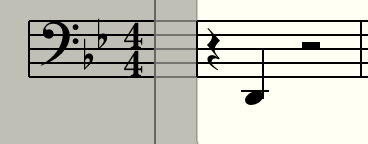
\includegraphics[width=0.25\columnwidth]{Tuba_Fig1} 
	\caption{Tuba Figur 1}
\end{figure}

\begin{lstlisting}
d1 $ sound "[~ sn ~ ~]"
\end{lstlisting}

\subsubsection{Figuren}
\textbf{Figur 2}\\
Es wurde eine Figur über 2 Takte ermittelt. Instrumentalist bläst in dieser Figur in die Tuba ohne dass die Lippen vibrieren, um ein Rauschen zu erzeugen. Am Ende der Figur wurde eine Pause als Atempause angenommen. 

\begin{figure}[h]
	\centering 
	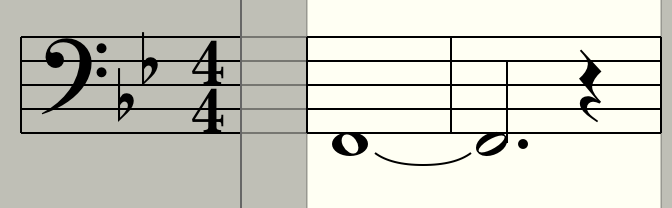
\includegraphics[width=0.25\columnwidth]{Tuba_Fig2} 
	\caption{Tuba Figur 2}
\end{figure}

\noindent Für die Umsetzung wird ein Sample benötigt, welches über die Dauer von zwei Takten reicht. Um dieses nur aller 2 Takte abzuspielen damit sich mehre Instanzen des Samples nicht überlagern kann der Ausdruck \verb|loopAt 2| \cite{tid9} verwendet werden.
\begin{lstlisting}
d1 $ loopAt 2 $ sound "blasesoundTuba"
\end{lstlisting}

\noindent\textbf{Figur 3}\\
Analyse-Ergebnis: Wie Figur 1, hier allerdings kurzes tonloses Pusten stoßweise gespielt anstelle von Schlag auf Mundstück. Code analog zu Figur 1.\\

\noindent\textbf{Figur 4}\\
Analyse-Ergebnis: Tiefe Töne durch Tuba. Die Tonhöhe ist nahezu nicht erkennbar. Die Tonhöhe wurde jedoch durch die Analyse in Figur 6 ableitbar. Die gespielten Töne werden über den Verlauf von zwei Durchläufen der Figur langsam lauter.\\

\begin{figure}[h]
	\centering 
	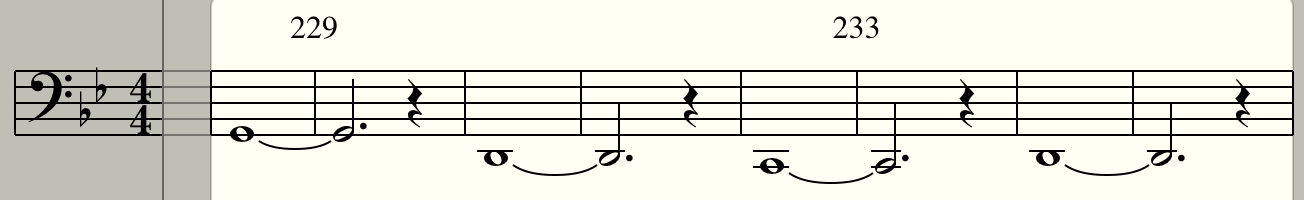
\includegraphics[width=0.7\columnwidth]{Tuba_Fig4} 
	\caption{Tuba Figur 4}
\end{figure}

\noindent Das lauter Werden der Töne über die Dauer von zwei Durchläufe der Figur wurde mit einem Pattern realisiert, welches dem \verb|# gain|-Effekt übergeben wurde.\cite{tid10} Um die lang ausgehaltenen Noten umzusetzen, wurde auf den Ausdruck ein Hall angewendet, wobei \verb|# room| die Lautstärke des Halls und \verb|# sz| die Größe des hallenden Raumes bedingt. \verb|# orbit 1| wird genutzt, um die ansonsten globale Wirkung des Hall-Effektes auf den vorangegangenen Ausdruck zu beschränken. \cite{tid11} 

\begin{lstlisting}
d1 $ slow 16 $ midinote "[43 38 36 38]*2" # s "superpiano" # room 0.85 # sz 0.8 # orbit 1 #gain "0.4 0.45 0.5 0.55 0.6 0.7 0.8 0.9"
\end{lstlisting}


\noindent\textbf{Figur 5}\\
Herausgehört wurde eine Figur analog zu Figur 4, jedoch kräftig gespielt.\\

\noindent\textbf{Figur 6}\\
Herausgehört wurde eine Figur analog zu Figur 5, jedoch maximal kraftvoll ausgespielt. Dabei werden die Töne jeweils eine Oktave höher gespielt, was die Tonhöhe der einzelnen Töne gut erkennbar macht.\\

\noindent Umsetzung in Tidal:
\begin{lstlisting}
d1 $ slow 8 $ midinote "55 50 48 50" # s "superpiano" # room 0.85 # sz 0.8 # orbit 1
\end{lstlisting}

\subsubsection{Klangbild}
\textit{Abschnitt bearbeitet von: Nico Mehlhose}\\
\noindent Bestandteile der Tuba: Eine Tuba, welche entartet, wie in den folgenden Figuren beschrieben, benutzt wird.\\
Art der Synthetisierung: Da die Tuba ein reales Musikinstrument ist, welches in dieser Form nicht im Supercollider enthalten ist,
werden hierfür selbst aufgenommene Samples benutzt. Die Samples werden für die entartete Benutzung in Tidal so manipuliert, dass sie die Sounds
nachempfinden. Des weiteren wurden Onlinesamples für die Figuren 4-6 benutzt.\cite{Orch}\\

\noindent\textbf{Figur 1}\\
 Sound: In dieser Figur wird auf das Mundstück der Tuba geschlagen. Der erzeugte Ton hört sich in etwa an wie eine Bass Drum ohne Bass.\\
Lösung: Um den eben beschriebenen Ton zu erzeugen, wurde die Bass Drum in Tidal mit \verb|Midinote| langgezogen. Damit nun dieser langgezogene Sound nicht über den gesamten Loop spielt, wurde eine High Hat mit \verb|Gain 0| eingefügt damit die HH keinen Sound macht. Anschließend muss der Ton der BD mit \verb|cut 1| geschnitten werden damit dieser bei der stummen HH aufhört zu spielen.
\begin{lstlisting}
d1 $ sound "~ bd hh ~" # cut 1 # midinote 15 #gain "1.3 0"
\end{lstlisting}

\noindent\textbf{Figur 2}\\
Sound: Bei Figur 2 ist das Klangbild vergleichbar eines Reifens der Luft verliert. Der Sound wurde selbst aufgenommen. Um den eben beschriebenen Ton nachzustellen wurde mit weit gespreizten Nasenflügeln ausgeatmet.\\
Lösung:Der \verb|room| sorgt dafür, dass sich der Sound nach einem größerem Gegenstand und nicht nach einer Nase anhört.
\begin{lstlisting}
d1 $ loopAt 2 $ sound "Atmen" #room 1 #orbit 1 # gain 1.3
\end{lstlisting}

\noindent\textbf{Figur 3}\\
Sound: Der Sound ist wie aus Figur 2 aber er wird mit mehr Druck und nicht durchgehend gespielt. Erstellt wurde der Sound durch das anspielen von einem Handscheibenwischer mit hohlem Griff.\\
Lösung: \verb|Room| und \verb|Gain| haben hier den selben Effekt wie in Figur 2
\begin{lstlisting}
d1 $ sound "[~ Tuba ~ ~]" # room 0.4 #orbit 1 # gain 1.1
\end{lstlisting}
\noindent\textbf{Figur 4, 5, 6}\\
Sound: Die Tuba wird in Figur 4 mit absteigender Lautstärke gespielt. In Figur 5 und 6 wird sie mit gleichbleibender Lautstärke gespielt wobei jedoch die Lautstärke
zwischen den Figuren ansteigt.\\
Lösung Figur 4:
\begin{lstlisting}
d1 $ slow 16 $ midinote "[55 50 48 50]*2" # s "TubaOrch:20" # cut 1 #gain " 1 0.95 0.9 0.85 0.8 0.7 0.7 0.7"
\end{lstlisting}
Lösungen für Figuren 5 und 6 sind oben zu sehen.

\subsection{Instrument 5: Posaune}
\subsubsection{Figuren}
\textit{Abschnitt bearbeitet von: Raphael Drechsler}\\

\noindent\textbf{Figur 1}\\
Herausgehört wurde eine Figur über einen Takt. In der Figur erfolgt ein kurzes, tonloses Pusten in die Posaune. Dieses wird Stoßweise gespielt und als rhythmisches Element auf letzte Achtelnote im Takt eingesetzt.
\begin{figure}[h]
	\centering 
	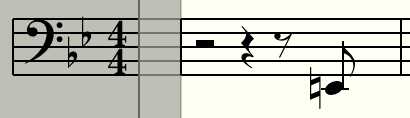
\includegraphics[width=0.25\columnwidth]{Posaune_Fig1} 
	\caption{Posaune Figur 1}
\end{figure}

\noindent Umsetzung in Tidal:
\begin{lstlisting}
d1 $ sound "[][[][~ sn]]"
\end{lstlisting}


\noindent\textbf{Figur 2}\\
Zu hören ist, dass die Figur ein Rauschen analog zur Figur 2 der Tuba umfasst. Der Code gestaltet sich entsprechend.
\begin{lstlisting}
d1 $ loopAt 2 $ sound "blasesoundPosaune"
\end{lstlisting}

\subsubsection{Klangbild}
\textit{Abschnitt bearbeitet von: Nico Mehlhose}\\

\noindent 
Bestandteile der Posaune: Gewöhnliche Posaune, welche aber entartet benutzt wird.\\
Art der Synthetisierung: Da die Posaune ein reales Musikinstrument ist, welches in dieser Form nicht im Supercollider enthalten ist,
werden hierfür Samples benutzt. Die Samples werden eigens dafür aufgenommen. Die Sound werden wie bei der Tuba erzeugt.\\

\noindent\textbf{Figur 1}\\
 Sound: In dieser Figur wird auf das Mundstück der Posaune stoßartig angespielt.\\
Lösung:\verb|room| bzw. \verb|gain| werden hier benutzt damit die Sounds sich nach einem größeren Hohlkörper und nicht nach einem Scheibenwischer anhören.
\begin{lstlisting}
d1 $ sound "[][[][~ Posaune]]" # room 0.3 #orbit 1 # gain 1.2
\end{lstlisting}

\noindent\textbf{Figur 2}\\
Sound: Ähnlich zu Figur 3 der Tuba allerdings ist dieser Sound weniger tief.\\
Lösung: Für die geringere Tiefe des Sounds wurde der Hall der Posaune angepasst.
\begin{lstlisting}
d1 $ loopAt 2 $ sound "Atmen" #room 0.6 #orbit 1 #gain 1.1
\end{lstlisting}

\subsection{Instrument 6: Violine}
\subsubsection{Figuren}
\textit{Abschnitt bearbeitet von: Raphael Drechsler}\\

\noindent\textbf{Figur 1}\\
Herausgehört wurde die folgende Figur über 16 Takte.
\begin{figure}[h]
	\centering 
	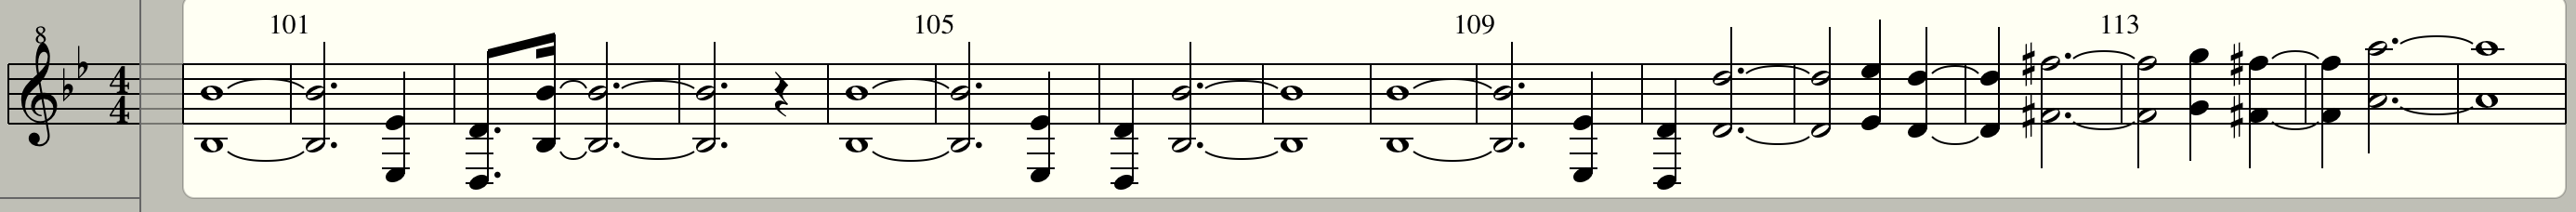
\includegraphics[width=0.99\columnwidth]{Violin_Fig1} 
	\caption{Violine Figur 1}
\end{figure}

\noindent Die Noten der Figur werden oktaviert gespielt. Der Einfachheit halber wurden nur die gut hörbaren hohen töne umgesetzt. Um jeweils einen Ton zu einem Zeitpunkt zu hören, werden die abgespielten Samples mithilfe des Ausdrucks \verb|# cut 1| immer dann gestoppt, sobald sie für den nächsten Ton abgespielt werden.\cite{tid12}

\begin{lstlisting}
d1 $ slow 4 $ cat [
midinote "[82][][][][][][][75][74][82][][][][][][]" # s "gtr",
midinote "[82][][][][][][][75][74][82][][][][][][]" # s "gtr",
midinote "[82][][][][][][][75][74][86][][][][][87][86]" # s "gtr",
midinote "[][90][][][][][91][90][][93][][][][][][]" # s "gtr"
] #cut 1 # room 0.85 # sz 0.8 # orbit 1 
\end{lstlisting}\

\noindent\textbf{Figur 2}\\
Analyse-Ergebnis:
\begin{figure}[h]
	\centering 
	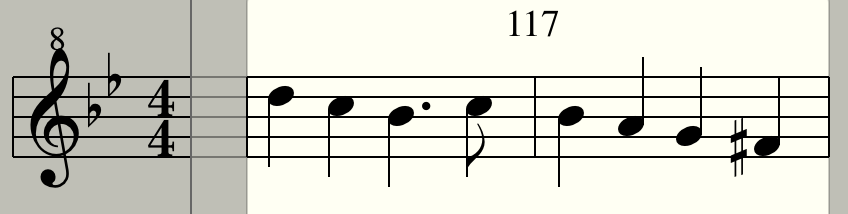
\includegraphics[width=0.3\columnwidth]{Violin_Fig2} 
	\caption{Violine Figur 2}
\end{figure}

\noindent Umsetzung in Tidal:
\begin{lstlisting}
d1 $ slow 2 $ midinote "[[86][84][82][[][84]]][82 81 79 78]" # s "gtr" #cut 1 # room 0.85 # sz 0.8 # orbit 1
\end{lstlisting}

\noindent\textbf{Weitere Figuren}\\
Im hinteren Teil des Stückes treten weitere Figuren der Violine auf. Da deren Umsetzung jedoch keinen signifikanten Unterschied in der Performance ausmacht wurde auf die Analyse und Synthese dieser Figuren verzichtet.

\subsubsection{Klangbild}
\textit{Abschnitt bearbeitet von: Nico Mehlhose}\\

\noindent 
Art der Synthetisierung: Hierfür wurden Samples Online gesucht da wir möglichst viele verschiedene Arten der Soundeinbindung abdecken wollten. Dabei wurde ein großer Datenbestand von Orchesterinstumenten gefunden.\cite{Orch} Des weiteren wäre es mit zusätzlichem Zeitaufwand verbunden gewesen jedes Instrument über den SuperCollider zu synthetisieren, weshalb Sound Samples für dieses Instrument gewählt wurden.\\

\noindent\textbf{Figur 1}\\
Sound: In dieser Figur steigt die Violine leise in das Stück ein und wird über die Zeit immer lauter, wodurch sie schlussendlich im zweiten Teil 
zum Hauptinstrument des Abschnittes wird. Im ersten Teil wird die Violine etwas quitschend und langsam gespielt. Teil zwei besteht aus einem hektisch aber sauber gespielt Part.\\
Problem: Die Violine muss in unserer Vorführung diesen gleichmäßigen Anstieg der Lautstärke vollführen, ohne merkliche Sprünge zu machen.\\
Lösung: Violine:5 ist ein Soundsample in dem eine Violine zu hören ist welche \textit{sustain} gespielt wird.
\begin{lstlisting}
d1 $ slow 4 $ cat [
midinote "[52][][][][][][][45][44][52][][][][][][]" # s "Violine:5",
midinote "[52][][][][][][][45][44][52][][][][][][]" # s "Violine:5",
midinote "[52][][][][][][][45][44][56][][][][][57][56]" # s "Violine:5",
midinote "[][60][][][][][61][60][][63][][][][][][]" # s "Violine:5"
] #cut 1 #speed 1.2 # sz 0.8 # orbit 1 # room 0.85 #gain 0.9
\end{lstlisting}
\noindent\textbf{Figur 2}\\
Sound: Wenn die Violine in diese Figur übergeht ist sie das Hauptinstrument des Stückes. Die Violine wird hierbei sehr hektisch aber im Gegensatz zu Figur 1 sauber gespielt.\\
Lösung: Violine:6 ist eine Violine die \textit{tremolo} gespielt wird.
\begin{lstlisting}
d1 $ slow 2 $ midinote "[[61][59][57][[][59]]][57 56 54 53]" # s "Violine:6" #cut 1 # room 0.85 # sz 0.8 # orbit 1
\end{lstlisting}

\subsection{Instrument 7: Chello}
\subsubsection{Figuren}
\textit{Abschnitt bearbeitet von: Raphael Drechsler}\\

\noindent\textbf{Figur 1}\\
Analyse-Ergebnis:
\begin{figure}[h]
	\centering 
	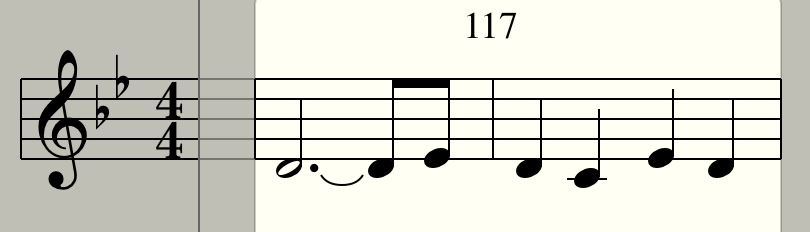
\includegraphics[width=0.3\columnwidth]{Chello_Fig1} 
	\caption{Chello Figur 1}
\end{figure}

\noindent Umsetzung in Tidal:
\begin{lstlisting}
d1 $ slow 2 $ midinote "[[74][][][[][75]]][74 72 75 74]" # s "gtr" #cut 1 # room 0.85 # sz 0.8 # orbit 1
\end{lstlisting}

\noindent\textbf{Figur 2}\\
Analyse-Ergebnis:
\begin{figure}[h]
	\centering 
	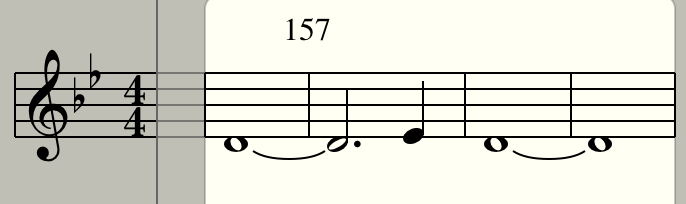
\includegraphics[width=0.3\columnwidth]{Chello_Fig2} 
	\caption{Chello Figur 2}
\end{figure}

\noindent Umsetzung in Tidal:
\begin{lstlisting}
d1 $ slow 4 $ midinote "[[62][[][][][63]]][62]" # s "gtr" #cut 1 # room 0.85 # sz 0.8 # orbit 1
\end{lstlisting}

\noindent\textbf{Weitere Figuren}\\
Analog zur Violine existieren im hinteren Teil des Stücks weitere Figuren, auf deren Analyse und Synthese ebenfalls verzichtet wurde.

\subsubsection{Klangbild}
\textit{Abschnitt bearbeitet von: Nico Mehlhose}\\

\noindent 
Art der Synthetisierung: Das Cello wird, wie auch die Violine, über die Samples synthetisiert\cite{Orch}, welches anschließend in den SuperCollider eingefügt werden.\\

\noindent\textbf{Figur 1}\\
Lösung:
\begin{lstlisting}
d1 $ slow 2 $ midinote "[[50][][][[][51]]][50 48 51 50]" # s "Cello:1" #cut 2 # room 0.85 # sz 0.8 # orbit 1 #gain 0.7
\end{lstlisting}
\noindent\textbf{Figur 2}\\
Lösung:
\begin{lstlisting}
d1 $ slow 4 $ midinote "[[50][[][][][51]]][50]" # s "Cello:2" #cut 2 # room 0.85 # sz 0.8 # orbit 1 #gain 0.7
\end{lstlisting}

\subsection{Instrument 8: Harfe}
\subsubsection{Figuren}
\textit{Abschnitt bearbeitet von: Raphael Drechsler}\\

\noindent\textbf{Figur 1}\\
Die Rhythmik sowie die Tonhöhe der zweitaktigen Figur ließen sich nicht ohne weiteres bestimmen. Zur Reduzierung des Arbeitsaufwandes wurde für die Figur die folgende Annahme getroffen. 
\begin{figure}[h]
	\centering 
	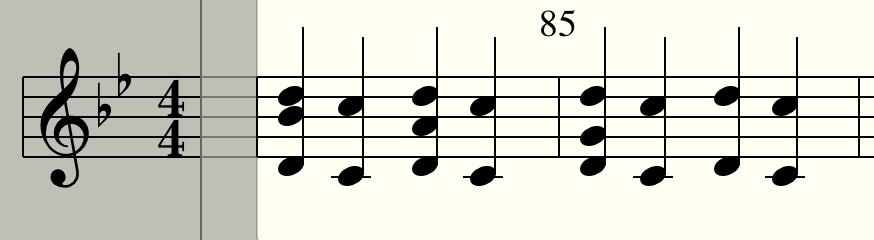
\includegraphics[width=0.3\columnwidth]{Harp_Fig1} 
	\caption{Harfe Figur 1}
\end{figure}

\noindent Umsetzung in Tidal:
\begin{lstlisting}
d1 $ stack [
  midinote "[74 72]*2" # s "gtr",
  midinote "[62 60]*2" # s "gtr",
  cat [
    midinote "70 69" # s "gtr",
    midinote "67" # s "gtr",
    midinote "70 69" # s "gtr",
    midinote "66" # s "gtr"
  ]
] 
\end{lstlisting}



\subsubsection{Klangbild}
\textit{Abschnitt bearbeitet von: Nico Mehlhose}\\
\noindent Bestandteile der Harfe: Harfe\\
Art der Synthetisierung: Die Harfe wird mit Samples\cite{Orch} synthetisiert da diese nicht über die SuperCollidertöne synthetisierbar ist.\\
Sound: Die Harfe wird in ihren Teilen sehr dominant gespielt.\\
Lösung:
\begin{lstlisting}
d1 "i8" $ slow 2 $ stack [
  midinote "[57 55]*4" # s "Harp:13",
  midinote "[45 43]*4" # s "Harp:13",
  slow 2 $ fastcat [
    midinote "53 52" # s "Harp:13",
    midinote "50" # s "Harp:13",
    midinote "53 52" # s "Harp:13",
    midinote "49" # s "Harp:13"
  ]
] #speed 2 # room 0.5 # orbit 1 #gain 0.9
\end{lstlisting}


\subsection{Instrument 9: Flügel}
\subsubsection{Figuren}
\textit{Abschnitt bearbeitet von: Raphael Drechsler}\\

\noindent\textbf{Figur 1}\\
Analyse-Ergebnis:
\begin{figure}[h]
	\centering 
	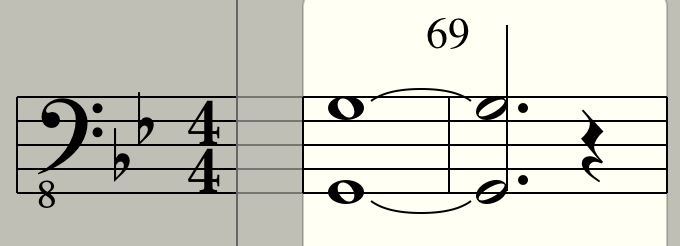
\includegraphics[width=0.3\columnwidth]{Flug_Fig1} 
	\caption{Flügel Figur 1}
\end{figure}
\noindent Umsetzung in Tidal:
\begin{lstlisting}
d1 $ slow 2 $ stack[midinote "43 " #s "superpiano", midinote "55 " #s "superpiano"]
\end{lstlisting}

\noindent \textbf{Figur 2}\\
Analyse-Ergebnis:\\
\begin{figure}[h]
	\centering 
	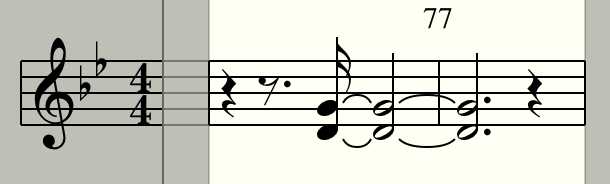
\includegraphics[width=0.3\columnwidth]{Flug_Fig2} 
	\caption{Flügel Figur 2}
\end{figure}\\
\noindent Umsetzung in Tidal:
\begin{lstlisting}
d1 $ slow 2 $ stack[
  midinote "[[][[][][][67]][][]][]" #s "superpiano",
  midinote "[[][[][][][62]][][]] []" #s "superpiano"
] # room 0.5 # sz 0.83 # orbit 1
\end{lstlisting}

\noindent \textbf{Figur 3}\\
Analyse-Ergebnis:
\begin{figure}[h]
	\centering 
	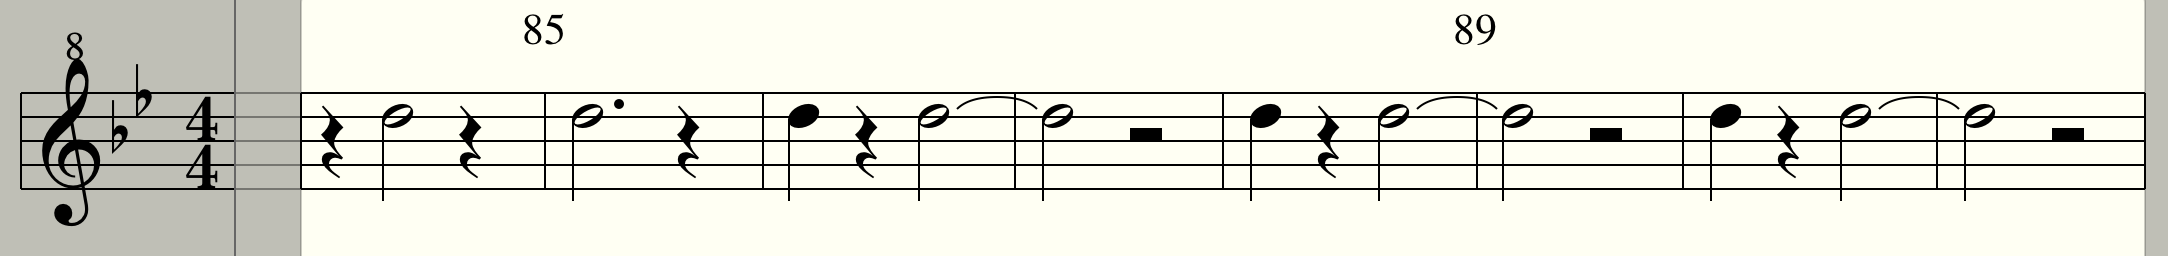
\includegraphics[width=0.8\columnwidth]{Flug_Fig3} 
	\caption{Flügel Figur 3}
\end{figure}

\noindent Umsetzung in Tidal:
\begin{lstlisting}
d1 $ slow 2 $ midinote "[86 ~][86][~] [~] " # s "superpiano"  # room 0.5 # sz 0.83 # orbit 1 #gain "<0.65 0.7 0.75 0.8>"
\end{lstlisting}


\noindent \textbf{Figur 4}\\
Analyse-Ergebnis:
\begin{figure}[h]
	\centering 
	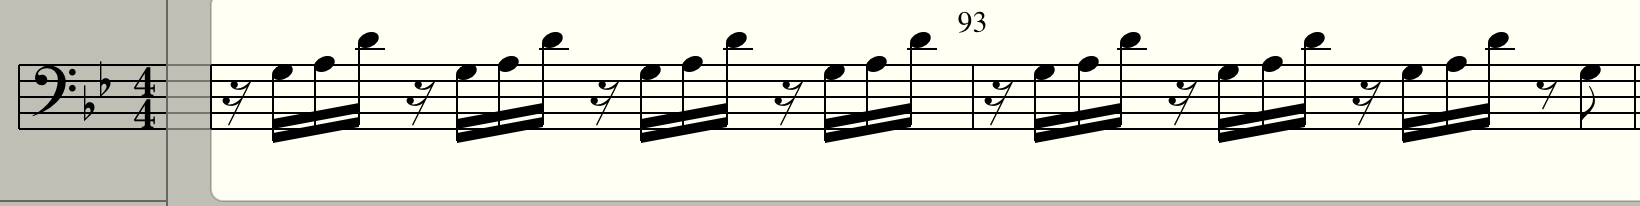
\includegraphics[width=0.9\columnwidth]{Flug_Fig4a} 
	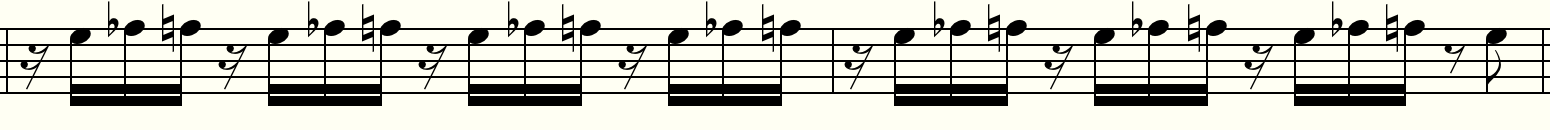
\includegraphics[width=0.9\columnwidth]{Flug_Fig4b} 
	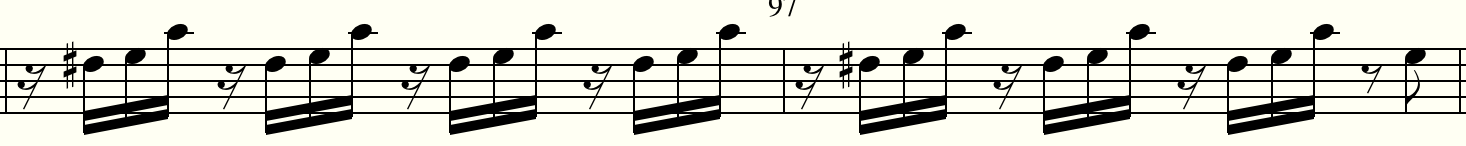
\includegraphics[width=0.9\columnwidth]{Flug_Fig4c} 
	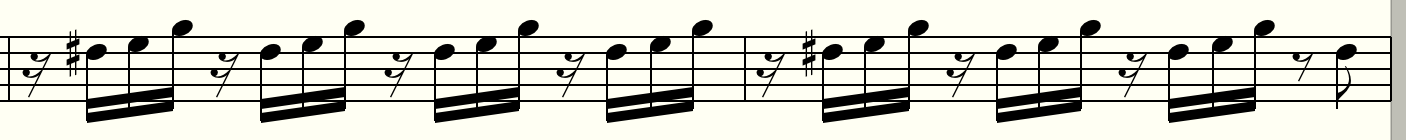
\includegraphics[width=0.9\columnwidth]{Flug_Fig4d} 
	\caption{Flügel Figur 4}
\end{figure}

\noindent Umsetzung in Tidal:
\begin{lstlisting}
d1 $ slow 2 $ cat [
midinote "~ 67 69 74 ~ 67 69 74 ~ 67 69 74 ~ 67 69 74 ~ 67 69 74 ~ 67 69 74 ~ 67 69 74  ~ ~ 67 ~ " # s "superpiano",
midinote "~ 67 68 69 ~ 67 68 69 ~ 67 68 69 ~ 67 68 69 ~ 67 68 69 ~ 67 68 69 ~ 67 68 69  ~ ~ 67 ~ " # s "superpiano",
midinote "~ 66 67 72 ~ 66 67 72 ~ 66 67 72 ~ 66 67 72 ~ 66 67 72 ~ 66 67 72 ~ 66 67 72  ~ ~ 67 ~ " # s "superpiano",
midinote "~ 66 67 70 ~ 66 67 70 ~ 66 67 70 ~ 66 67 70 ~ 66 67 70 ~ 66 67 70 ~ 66 67 70  ~ ~ 66 ~ " # s "superpiano"
]
\end{lstlisting}

\noindent \textbf{Figur 5}\\
Analyse-Ergebnis:
\begin{figure}[h]
	\centering 
	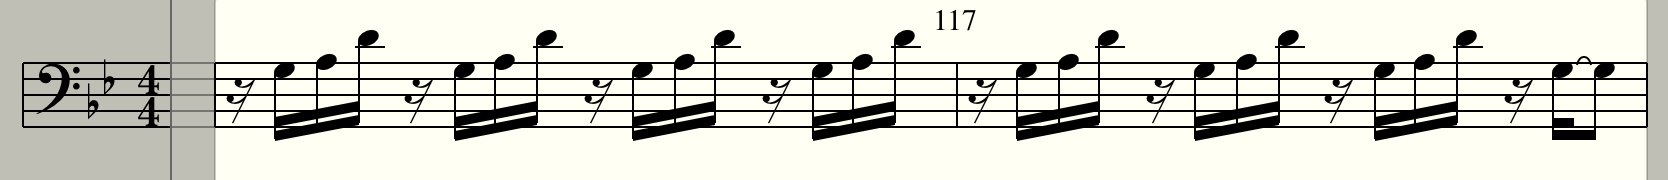
\includegraphics[width=0.9\columnwidth]{Flug_Fig5} 
	\caption{Flügel Figur 5}
\end{figure}

\noindent Umsetzung in Tidal:
\begin{lstlisting}
d1 $ slow 2 $ midinote "~ 67 69 74 ~ 67 69 74 ~ 67 69 74 ~ 67 69 74 ~ 67 69 74 ~ 67 69 74 ~ 67 69 74  ~ ~ 67 ~ " # s "superpiano"
\end{lstlisting}


\subsubsection{Klangbild}
\textit{Abschnitt bearbeitet von: Nico Mehlhose}\\

\noindent Bestandteile des Flügels: Flügel\\
Art der Synthetisierung: Der Flügel wurde mittels dem SuperCollider syntetisiert. Dazu wurde die Funktion \textit{OteyPianos} benutzt, welche einen Pianoartigen klang besitzt. Der restliche Teil der geschriebenen Funktion schneidet die Höhen etwas heraus und gibt dem Klang etwas mehr Tiefe. 
\begin{lstlisting}
(
SynthDef(\piano, { |out=0, freq= 391.995,gate=1, amp=0.5,rho=1|
    var son = OteyPiano.ar(freq, amp, rho:rho)*EnvGen.ar(Env.asr(0,1,0.1),gate,doneAction:2);
    Out.ar(out, Pan2.ar(son * 0.1, LinLin.kr(freq,36.midicps,90.midicps,-0.75,0.75)));
}).play(s);
)
\end{lstlisting}
\noindent \textbf{Figur 1}\\
Sound: Der Sound der Figur wird zur Einleitung in den ersten Hauptabschnitt benutzt. Dabei werden die Tasten des Flügels 
schnell gedrückt um einen möglichst lauten Ton hervorzubringen.\\
Lösung: In dieser Figur wurden die zwei Töne die stark angespielt wurden bereits per Audacity zusammengeschnitten um Code einzusparen.
\begin{lstlisting}
d1 $ slow 2 $ sound "[K]" # room 0.2 #orbit 1 # gain 1.3
\end{lstlisting}
\noindent \textbf{Figur 2}\\
Sound: Der Sound der Figur wird zu der Hinführung in den ersten Hauptabschnitt benutzt. Dabei werden die Tasten des Flügels 
schnell gedrückt um einen möglichst lauten Ton hervorzubringen.\\
Lösung:
\begin{lstlisting}
d1 $ slow 8 $ sound "[[][[][][][K:1]][][]] [] [] [] [[][[][][][K:1]][][]] [] [] []" # room 0.2 #orbit 1 #gain 1.2
\end{lstlisting}
\noindent \textbf{Figur 3}\\
Sound: Der Flügel wird gefühlvoller angespielt um im Einklang mit der Harfe zu stehen.
Lösung: \verb|speed 2| wird hier benutzt damit das Soundsample des Flügels eine Oktave höher gespielt wird.
\begin{lstlisting}
d1 $ slow 2 $ sound "[K:2 ~][K:2][~] [~] "  #speed 2 #room 0.4 #orbit 1 #gain 1.5
\end{lstlisting}
\noindent \textbf{Figur 4}\\
Sound: Der Flügel wird in dieser Figur normal angespielt und führt den Zuhörer zu dem Höhepunkt des ersten Haupteiles welcher von der Violine gespielt wird.\\

\begin{tabular}{lcr}
Midinote Superpiano & Soundsample K: \\ 
66&7\\
67&3\\
68&6\\
69&4\\
70&9\\
72&8\\
74&5\\
\end{tabular}\\

\noindent Melodie: siehe Melodiepart Figur 4 Flügel\\

\noindent \textbf{Figur 5}\\
Sound: In der Figur wird der Flügel normal gespielt.\\
Lösung:\\
siehe Tabelle und Melodie Figur 5 Flügel

\subsection{Instrument 10: Moog Syntheziser}
\subsubsection{Figuren}
\textit{Abschnitt bearbeitet von: Raphael Drechsler}\\

\noindent\textbf{Figur 1}\\
Herausgehört wurde der folgende Basslauf über acht Takte.\\
\begin{figure}[h]
	\centering 
	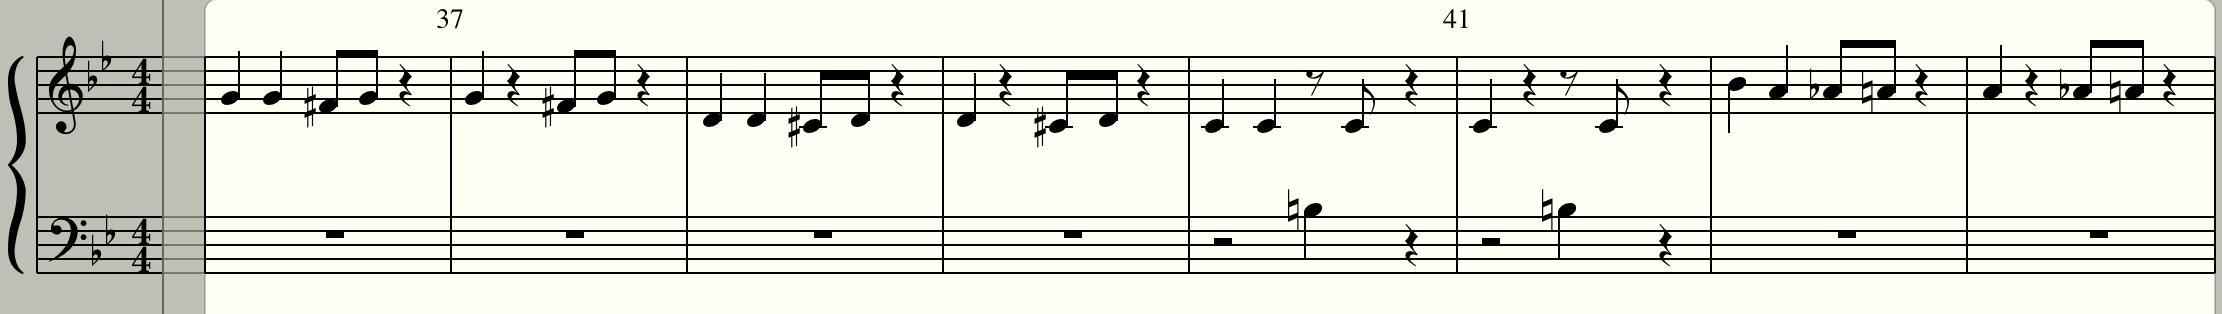
\includegraphics[width=1\columnwidth]{Bass_Fig1} 
	\caption{Moog Figur 1}
\end{figure}

\noindent Umsetzung in Tidal:
\begin{lstlisting}
d1 $ slow 2 $ cat [
  midinote "[[55 55][54 55 ~ ~]]*2" # s "moog",
  midinote "[[50 50][49 50 ~ ~]]*2" # s "moog",
  midinote "[[48 48][47 48 ~ ~]]*2" # s "moog",
  midinote "[[58 57][56 57 ~ ~]]  [[57 ~][56 57 ~ ~]]" # s "moog" 
] # cut 1
\end{lstlisting}

\noindent\textbf{Figur 2}\\
Herausgehört wurde der folgende Basslauf über einen Takt.
\begin{figure}[h]
	\centering 
	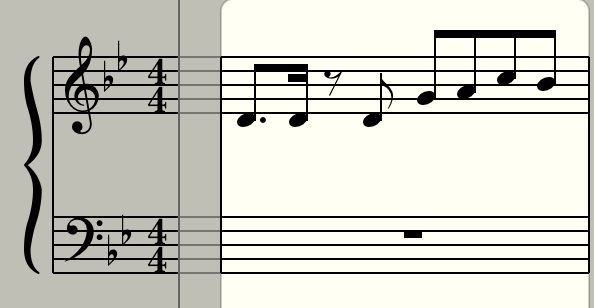
\includegraphics[width=0.3\columnwidth]{Bass_Fig2} 
	\caption{Moog Figur 2}
\end{figure}

\noindent Umsetzung in Tidal:
\begin{lstlisting}
d1 $ midinote "[[[[50 ~ ~ 50]][~ 50]][55 57 60 58]]" # s "moog" # cut 1
\end{lstlisting}

\subsubsection{Klangbild}
\textit{Abschnitt bearbeitet von: Nico Mehlhose}\\

\noindent Bestandteile des Moogs: Keyboard, PC, Mischboard\\
Art der Synthetisierung: Der Moog wird mittels dem SuperCollider programmiert. Der SuperCollider besitzt die Funktion, welche einen Moog synthetisieren kann.
Dies ist die \textit{BMoog}-Funktion welche im folgendem Codebeispiel zu sehen ist. Als nächstes müssen nurnoch die Sounds für die verschiedenen
Frequenzen aufgenommen, geschnitten und eingefügt werden.
\begin{lstlisting}
x=(
SynthDef(\moog, {
	arg freq=102, width=0.5, mul=0.5, freq2=300, q=0.2, mode=0;
	var moog ;
	
		moog=BMoog.ar(Pulse.ar(freq,width,  mul),freq2, q, mode, mul:0.2);
		
		
		Out.ar(0, moog);
		Out.ar(1, moog);
	
}).play
)
\end{lstlisting}
Der eingefügte Moog Sound schwingt in beiden Figuren auf 66 Hz und wurde mittels dem \verb|Midinote| Operator manipuliert.\\
\noindent\textbf{Figur 1}\\
Lösung:
\begin{lstlisting}
p "i10" $ slow 2 $ cat [
  midinote "[[55 55][54 55 ~ ~]]*2" # s "BBFMoog:6",
  midinote "[[50 50][49 50 ~ ~]]*2" # s "BBFMoog:6",
  midinote "[[48 48][47 48 ~ ~]]*2" # s "BBFMoog:6",
  midinote "[[58 57][56 57 ~ ~]]  [[57 ~][56 57 ~ ~]]" # s "BBFMoog:6"
] # cut 1 #speed 2 #gain 0.9
\end{lstlisting}
\noindent\textbf{Figur 2}\\
Lösung:
\begin{lstlisting}
p "i10" $ midinote "[[[[50 ~ ~ 50]][~ 50]][55 57 60 58]]" # s "BBFMoog:6" # cut 1 #speed 2 #gain 1.0
\end{lstlisting}


\section{Performance}
\subsection{Umsetzung der Performance}
\textit{Abschnitt bearbeitet von: Raphael Drechsler}\\

\noindent Nachdem die einzelnen Figuren aller Instrumente durch das vorangegangene Kapitel als Tidal-Code umgesetzt sind, soll nun die vorführbare Performance aus den einzelnen Teilen zusammengesetzt werden. Dabei soll im Wesentlichen die in Abbildung 1 gezeigte globale Struktur des Liedes nachempfunden werden.\\
Ein erster gedanklicher Ansatz bei der Umsetzung bestand in der Nutzung von mehreren Tidal-Connections. Tidal stellt 16 Verbindungen zum SuperDirt-Synthesizer bereit\cite{tid14}, daher kann jedes Instrument auf einer separaten Verbindung gespielt werden. Durch das Auswerten einzelner Zeilen während der Vorführung lassen sich somit die Figuren pro Instrument um- und abschalten. Der Code der Performance würde sich wie folgt darstellen.

\begin{lstlisting}
d1 $ --Tidal-Code Drum-Figur 1
d1 $ --Tidal-Code Drum-Figur 2
d1 $ --Tidal-Code Drum-Figur n
d1 $ silence
...
d2 $ --Tidal-Code Marimba-Figur 1
d2 $ --Tidal-Code Marimba-Figur 2
d2 $ silence
...
d9 $ --Tidal-Code Moog Figur 2
d9 $ silence
\end{lstlisting}

\noindent Dabei ergibt sich jedoch das Problem, dass pro Zeitpunkt immer nur eine Änderung für ein Instrument ausgewertet werden kann. In der angestrebten Performance finden jedoch zu einzelnen Zeitpunkten mehrere Änderungen statt. So wird zum Beispiel beim Übergang von Part 4 in Part 5 der Bass (Moog-Synthesizer) pausiert, während Piano, Harfe und Marimba zeitgleich eine neue Figur zu spielen beginnen.\\

\noindent Um mehrere Instrumente innerhalb einer Code-Auswertung dazuschalten oder muten zu können, wurde die Implementierung der Performance an die in der Tidal Userbase beschriebene Vorgehensweise für das Stummschalten einzelner Instrumente angepasst.\cite{tid13} Dazu wurden für alle Instrumente dieselbe Tidal-Connection \verb|d1| genutzt und die einzelnen Figuren mithilfe des \verb|stack|-Ausdrucks miteinander verbunden. Dabei wurden alle Parts, die abschaltbar sein sollen in eine eigene Zeile geschrieben. Über die Nutzung des Tasten-Kurzbefehls für das Aus- bzw. Einkommentieren einzelner Zeilen im Code-Editor und das erneute Auswerten des gesamten Befehls, lassen sich somit einzelne Bestandteile in kurzer Zeit muten und wieder aktivieren.\\
Als Code-Editor wurde Atom verwendet. Um in Atom den gesamten Code des Ausdrucks trotz langer Zeilen im Bild zu behalten, muss im Einstellungsmenü unter dem Menüpunkt \textit{Editor} über das Setzen des Kontrollkästchens \textit{Soft Wrap} der Zeilenumbruch aktiviert werden.\cite{atom1}. \\

\noindent Um das Vorgehen für das Dazu- und Umschalten einzelner Spuren zu illustrieren, soll zunächst der Code für den ersten Part gezeigt und dessen Verwendung beschrieben werden.

\lstset{
	numbers=left,
}
\lstinputlisting[language=Haskell]{Figures/part1.hs}

\noindent Zunächst wird der Code ausgeführt und die Performance beginnt.
Entsprechend der globalen Struktur (Abbildung 1) wird nach einigen durchlaufenen Takten Figur 1 der Posaune gestartet. Dazu wird die Kommentierung der Zeile 13 per Tastenkurzbefehl aufgehoben und der gesamte Ausdruck ebenfalls per Tastenkurzbefehl erneut ausgewertet. Nach weiteren durchlaufenen Takten wechselt die Marimba von Figur 1 zu Figur 2. Diese Figuren unterscheiden sich den gespielten Kuhglocken. Der Code für diese befindet sich in Zeile 8. Folglich muss zum gewünschten Zeitpunkt Zeile 8 ent-kommentiert und der gesamte Ausdruck erneut ausgewertet werden.\\
Im Code zu Part 1 findet sich für die Schlagzeugspur in Zeile 4 ein Ausdruck \verb|# gain 0.4|. Dieser soll genutzt werden um über das Vergrößern des Parameters in den ersten Takten von Part 1 live die Lautstärke der Schlagzeug-Figur anwachsen zu lassen, um die ansteigende BD nachzuempfinden. Zudem finden sich in der Performance vereinzelt weitere genutzte Effekte. So werden zum Beispiel die Figuren der Tuba und der Posaune mithilfe des \verb|#pan|-Effektes\cite{tid15} im Stereo-Kanal nach links und rechts verschoben um den Gesamtklang der Performance zu verbessern.\\

\noindent Das hohe Maß von wiederkehrenden und gleichbleibenden Figuren kann genutzt werden, um mehrere Parts des Liedes in einem Ausdruck zusammenzufassen. Dies wird im nachfolgend skizzierten Ausdruck für Part 2,3 und 4 deutlich. 

\lstinputlisting[language=Haskell]{Figures/part2.hs}
\lstset{
	numbers=none,
}

\noindent Dabei sind alle vorkommenden Figuren eines Instrumentes jeweils untereinander geschrieben. Entsprechend der globalen Struktur ist pro Wechsel der Parts die Kommentierung per Tastenkurzbefehl derartig anzupassen, dass nur die gewünschten Figuren als Code ausgewertet werden. Zur besseren Übersichtlichkeit während der Performance sind alle gleichbleibenden Figuren im unteren Teil (im Auszug ab Zeile 18) zusammengefasst.\\

\noindent Der vollständige Code der Performance findet sich in der digitalen Anlage.

\subsection{Abwesenheit von Sounds}
\textit{Abschnitt bearbeitet von: Nico Mehlhose}\\

\noindent In der Livevorführung sind nicht alle erzeugten Sounds zu hören, welche von uns eigens für die Klangsynthese aufgenommen wurden. Dieser Abschnitt soll erklären wieso einige Sounds von uns nicht verwendet werden.\\
In Figur 2 der Marimba werden Kuh-Glocken per Zufall angespielt. Die Glockensounds wurden im SuperCollider erzeugt mit folgendem Code:
\begin{lstlisting}
-Code Marimba-
(
Pbind(
	\instrument, \bell,
	\fs, Pseq( (60..72), 1).midicps,
	\t60, 3,
	\pitchy, 2,
	\dur, 1
).play;
)
\end{lstlisting}
Durch eben gezeigten Code wurden 10 Glockensounds erzeugt. Bei dem zusammenfügen der Liveperformance fiehl uns aber auf das die Sounds das Klangbild zerstören, da diese viel zu hell waren und eher dumpf klingen müssen.\\
Die nächsten Sounds die nicht eingebunden wurden, waren die des Moogs. Für den Moog wurden extra die Frequenzen mittels dem \textit{Sonic Visualiser}, welches ein kostenloses Programm zur Ansicht und Analyse von Audiodateien ist, ausgelesen.\cite{Sonic} Diese Frequenzen wurden dann im SuperCollider und dem im Moog gezeigten Code erzeugt, geschnitten und in unseren Code geschrieben. Bei der Zusammenführung der Performance hatte der Moog nicht die richtigen Frequenzen getroffen, was daran liegt das der Moog einen ca. 10 Hz großen Bereich in der Visualisierung angezeigt hat. Dies führte zu dem schlechten Klangbild. Um dieses Problem zu lösen wurde sich ein Referenzton aus den erzeugten Samples gesucht, der mit der Liveperformance von \textit{Brandt Brauer Frick} übereinstimmt. Mit diesem Referenzton wurde dann der Moog (Instrument 10) erzeugt. Die restlichen erzeugten Sounds für den Moog wurden als nächstes aus der Performance entfernt.\\
Alle eben genannten selbst erzeugten Töne sind unter \textit{Sounds/Eigene/Instrumentename} zu finden.\\
Der letzte Sound der nicht in der Lifeperformance zu finden ist, ist die erste Figur der Tuba. Es ist uns nicht gelungen einen ähnlichen Sound wie diesen zu erzeugen, aufzunehmen oder Sounds in Tidal so zu entfremden das sie diesem Sound nahe kommen und eine akzeptierbare Qualität besitzen. Das nächste was an diesen Sound herangekommen ist, ist der aus Figur 1 der Tuba. Dieser Sound hat jedoch das Problem, dass die Qualität des Sounds unzureichend war.Aus diesem Grund benutzen wir eine einfache Clap um diesen Ton nachzustellen, da es der Grundidee des Originalsounds am nächsten kommt.
\begin{lstlisting}
Benutzter Sound
p "i4" $ sound "[~ cp ~ ~]" #pan 0.2

Erstellter Sound
p "i4" $ sound "~ bd hh ~" # cut 1 # midinote 15 #gain "2 0"

\end{lstlisting}
\section{Gesang}\
\textit{Abschnitt bearbeitet von: Raphael Drechsler}\\

\noindent Neben der Umsetzung der einzelnen Instrumente wurden zusätzlich mit der Unterstützung einer Sängerin Gesangsaufnahmen angefertigt. Diese wurden ebenfalls SuperCollider als Sample zur Verfügung gestellt.\\
Hierbei galt es eine Herausforderung zu überwinden. Die Figuren des Gesangs sind acht Takte lang, starten jedoch nicht auf den ersten Schlag des ersten Taktes eines acht-Takte Intervalls; sie haben einen Auftakt.\\ Über das Berücksichtigen des Auftaktes bei der Aufnahme und mithilfe der folgenden Zeile Code können die acht Takte lange Samples für den Gesang mit dem Timing, welches dem Original entspricht, in der Performance verwendet werden.


\begin{lstlisting}
d1 $ slow 8 $ sound "[[[][[][[][VocP5]]]]]"
\end{lstlisting}

\section{Zusammenfassung}
\textit{Bearbeitet von Nico Mehlhose, Raphael Drechsler}\\

\noindent In diesem Dokument wurde zunächst aufgezeigt, weshalb sich für eine Umsetzung des Liedes \textit{Pretend} von \textit{Brand Brauer Frick} in Tidal anstatt in Euterpea entschieden wurde.\\ 
Die einzelnen Instrumente und deren Figuren wurden hinsichtlich ihrer Melodik, Rhythmik und ihres Klangbildes analysiert und entsprechend in Tidal Umgesetzt. Um ein originalgetreues Klangbild zu erzielen wurden dabei eigene Samples aufgenommen, Onlinesamples verwendet,  Sounds des SuperColliders manipuliert sowie eigene Sounds in SuperCollider geschrieben.\\
Die einzelnen Figuren der Instrumente wurden entsprechend der ermittelten globalen Struktur zu einer live ausführbaren Performance zusammengefügt. Dabei wurden die Lautstärken der Instrumente aufeinander angepasst, weitere Effekte zur Verbesserung des Gesamtklanges eingebracht und die zuvor angefertigten Gesangssamples eingefügt.\\

\noindent Die Tidal-Dateien \verb|BBF_instruments.tidal|, welche die Figuren der einzelnen Instrumente enthält und \verb|BBFhs.tidal|, welche die Performance enthält, sind zusammen mit den Sounds unter der folgenden URL verfügbar. \\
\url{https://github.com/MeisterXYZ/CM/tree/master/Code%2BSounds}
	
\pagebreak



%----------------------------------------------------------------------------------------
%	BIBLIOGRAPHY
%----------------------------------------------------------------------------------------

\renewcommand{\refname}{\spacedlowsmallcaps{Literatur/Quellen}} % For modifying the bibliography heading

\bibliographystyle{unsrt}

\bibliography{biblo.bib} % The file containing the bibliography

%----------------------------------------------------------------------------------------

\end{document}